% =========================================================================
% AAT — Figure: Driver-in-Snow as Worked AAT Instance (foundation panel, v2)
% Companion to: AAT preamble; cross-referenced across Part I Chs. 3-4,
% Part II Ch. 1, Appendix A multi-timescale section.
%
% Build:  pdflatex driver-snow-foundation.tex
%
% v2 changes (2026-05-15, per Joseph): single wiper blade (not two);
% trapezoid + swept arc as the central visual affordance (universal
% recognition); translation table corrected to use code-as-notation
% (not CS concepts); cleaner callouts.
% =========================================================================
\documentclass[border=10pt]{standalone}
\usepackage{tikz}
\usepackage{amsmath,amssymb}
\usepackage{array}
\usetikzlibrary{arrows.meta,calc,positioning,matrix}

\begin{document}
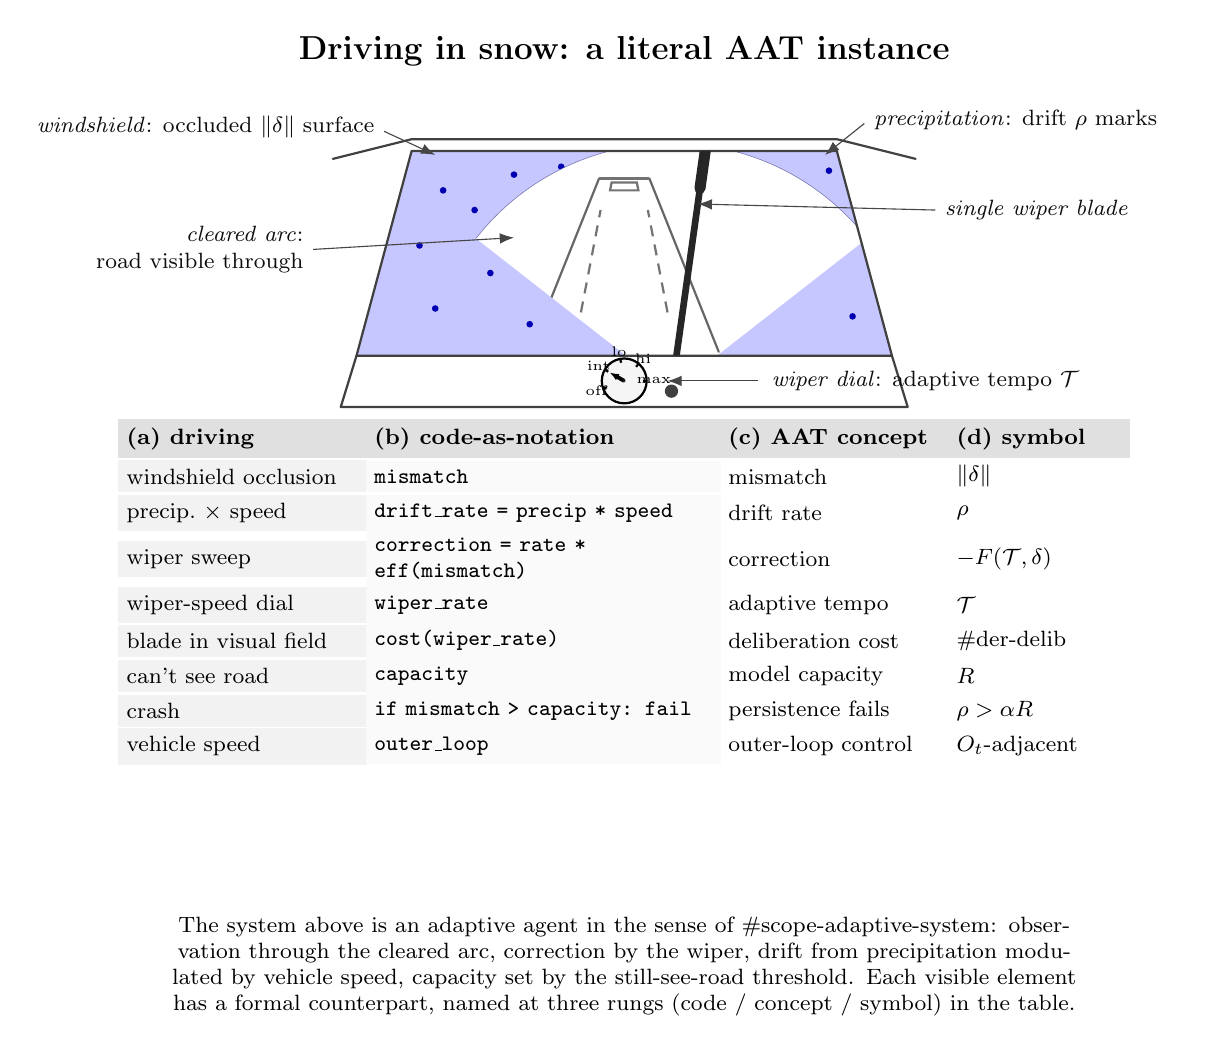
\begin{tikzpicture}[
    font=\small,
    >=Latex,
    frame/.style       = {thick, draw=black!75, line cap=round, line join=round},
    occluded/.style    = {fill=blue!22},
    cleared/.style     = {fill=white},
    wiper/.style       = {line width=2.4pt, draw=black!85, line cap=round},
    flake/.style       = {fill=blue!70!black},
    road/.style        = {thick, draw=black!60, line cap=round},
    lane/.style        = {thick, draw=black!55, dash pattern=on 4pt off 3pt},
    arc-edge/.style    = {very thin, draw=blue!35!black, opacity=0.5},
    callout/.style     = {-{Latex[length=1.8mm]}, thin, gray!55!black},
    callout-lbl/.style = {font=\footnotesize, gray!10!black}
  ]

% ====================================================
% Geometry parameters
% ====================================================
% Windshield trapezoid (driver POV from inside the cabin)
\def\wxBL{-3.4} \def\wyBL{0}     % bottom-left
\def\wxBR{3.4}  \def\wyBR{0}
\def\wxTL{-2.7} \def\wyTL{2.6}   % top-left (narrower)
\def\wxTR{2.7}  \def\wyTR{2.6}

% Wiper pivot (below the visible windshield, in the dashboard cowl;
% slightly right of center as in most LHD vehicles)
\def\px{0.6}  \def\py{-0.45}
\def\armL{3.15}     % wiper arm length

% Sweep angles (fan opens upward; corners remain unswept)
\def\sweepFrom{38}  % rest position (right side)
\def\sweepTo{142}   % extreme position (left side)
\def\armAt{82}      % current arm angle (just past vertical, mid-sweep)

% Windshield path (for re-use)
\def\windshield{(\wxBL,\wyBL) -- (\wxTL,\wyTL) -- (\wxTR,\wyTR) -- (\wxBR,\wyBR) -- cycle}

% Wiper-swept sector path (for re-use)
\def\sweptsector{(\px,\py) -- ($(\px,\py) + (\sweepFrom:\armL)$)
                  arc(\sweepFrom:\sweepTo:\armL) -- cycle}

% ====================================================
% LAYER 1: occluded background within windshield
% ====================================================
\begin{scope}
  \clip \windshield;

  \fill[occluded] (-4, -0.5) rectangle (4, 3.5);

  % Precipitation marks scattered throughout the windshield
  \foreach \x/\y in {%
      -2.8/2.35, -2.3/2.1,  -2.6/1.4,  -2.4/0.6,
      -1.9/1.85, -1.7/1.05, -1.4/2.3,  -1.2/0.4,
      -0.8/2.4,  -0.6/1.7,  -0.4/0.85,
       0.3/2.35,  0.5/0.95,
       0.9/2.0,   1.2/1.45,  1.4/2.4,   1.5/0.55,
       1.9/2.25,  2.0/1.7,   2.2/0.95,
       2.6/2.35,  2.8/1.45,  2.9/0.5
  } \fill[flake] (\x, \y) circle (1.2pt);

  % ----------------------------------------------------
  % LAYER 2: clear the wiper-swept sector (overlay white)
  % ----------------------------------------------------
  \fill[cleared] \sweptsector;

  % ----------------------------------------------------
  % LAYER 3: road through the cleared sector
  % ----------------------------------------------------
  \begin{scope}
    \clip \sweptsector;

    % Lane edges (perspective lines toward horizon)
    \draw[road] (-1.2, 0.05) -- (-0.32, 2.25);
    \draw[road] ( 1.2, 0.05) -- ( 0.32, 2.25);
    % Dashed center lane
    \draw[lane] (-0.55, 0.55) -- (-0.30, 1.85);
    \draw[lane] ( 0.55, 0.55) -- ( 0.30, 1.85);
    % Horizon
    \draw[black!55, thick] (-0.32, 2.25) -- (0.32, 2.25);
    % A faint distant vehicle suggestion
    \draw[thick, black!55] (-0.18, 2.10) -- (0.18, 2.10) -- (0.16, 2.20) -- (-0.16, 2.20) -- cycle;
  \end{scope}

  % Trace the leading-edge arc lightly so the eye perceives the sweep boundary
  \draw[arc-edge] ($(\px,\py) + (\sweepFrom:\armL)$)
       arc(\sweepFrom:\sweepTo:\armL);
\end{scope}

% ====================================================
% LAYER 4: windshield frame (outline)
% ====================================================
\draw[frame] \windshield;

% Cabin context: roof line above, dashboard below (with cowl where pivot lives)
\draw[frame, thick] (-3.7, 2.5) -- (-2.7, 2.75) -- (2.7, 2.75) -- (3.7, 2.5);
\draw[frame, thick] (-3.4, 0) -- (-3.6, -0.65) -- (3.6, -0.65) -- (3.4, 0);
% Pivot pin visible on the dashboard
\fill[black!75] (\px,\py) circle (2.4pt);

% ====================================================
% LAYER 5: single wiper blade (clipped to windshield, on top)
% ====================================================
\begin{scope}
  \clip \windshield;
  \draw[wiper] (\px,\py) -- ($(\px,\py) + (\armAt:\armL)$);
  % Blade tip emphasis (slight thickening at the end)
  \draw[wiper, line width=4pt, line cap=round]
     ($(\px,\py) + ({\armAt}:{\armL-0.55})$) -- ($(\px,\py) + (\armAt:\armL)$);
\end{scope}
% Pivot pin (outside the clip so it's clearly anchored to the dashboard)
\fill[black!75] (\px,\py) circle (2.0pt);

% ====================================================
% Wiper-speed dial (inset on dashboard)
% ====================================================
\begin{scope}[shift={(0, -0.32)}, scale=0.30]
  \draw[thick, fill=black!4] (0,0) circle (0.95);
  \foreach \ang/\lbl in {200/off, 150/int, 100/lo, 50/hi, 0/max} {
    \draw[thick] (\ang:0.78) -- (\ang:0.95);
    \node[font=\tiny, anchor=center] at (\ang:1.25) {\lbl};
  }
  \draw[line width=1.4pt, -{Latex[length=1.2mm]}] (0,0) -- (150:0.72);
  \fill[black!85] (0,0) circle (1.8pt);
\end{scope}

% ====================================================
% Callouts (sparse, well-placed)
% ====================================================
% windshield (the mismatch surface)
\draw[callout] (-3.05, 2.85) -- (-2.4, 2.55);
\node[callout-lbl, anchor=east] at (-3.05, 2.90)
   {\textit{windshield}: occluded $\lVert\delta\rVert$ surface};

% precipitation (drift source)
\draw[callout] (3.05, 2.95) -- (2.55, 2.55);
\node[callout-lbl, anchor=west] at (3.05, 3.00)
   {\textit{precipitation}: drift $\rho$ marks};

% wiper blade
\draw[callout] (3.95, 1.85) -- ($(\px,\py) + (\armAt:2.4)$);
\node[callout-lbl, anchor=west] at (3.95, 1.85)
   {\textit{single wiper blade}};

% swept arc (cleared region)
\draw[callout] (-3.95, 1.35) -- (-1.4, 1.50);
\node[callout-lbl, anchor=east, align=right] at (-3.95, 1.35)
   {\textit{cleared arc}: \\ road visible through};

% wiper dial
\draw[callout] (1.7, -0.32) -- (0.55, -0.32);
\node[callout-lbl, anchor=west] at (1.75, -0.32)
   {\textit{wiper dial}: adaptive tempo $\mathcal{T}$};

% ====================================================
% Translation table (below the schematic, 4 columns)
% ====================================================
\begin{scope}[yshift=-3.0cm]

  \matrix (T) [matrix of nodes,
               nodes={anchor=west, font=\footnotesize, inner sep=3pt,
                      minimum height=4mm},
               column 1/.style={nodes={text width=2.95cm, fill=black!5}},
               column 2/.style={nodes={text width=4.30cm, fill=black!2,
                                       font=\footnotesize\ttfamily}},
               column 3/.style={nodes={text width=2.70cm}},
               column 4/.style={nodes={text width=2.10cm}},
               row 1/.style={nodes={font=\footnotesize\bfseries, fill=black!12}},
               row sep=-\pgflinewidth,
               column sep=-\pgflinewidth
              ]
  {
    (a) driving & (b) code-as-notation & (c) AAT concept & (d) symbol \\
    windshield occlusion & mismatch                            & mismatch & $\lVert\delta\rVert$ \\
    precip.\ $\times$ speed & drift\_rate = precip * speed     & drift rate & $\rho$ \\
    wiper sweep & correction = rate * eff(mismatch)            & correction & $-F(\mathcal{T},\delta)$ \\
    wiper-speed dial & wiper\_rate                              & adaptive tempo & $\mathcal{T}$ \\
    blade in visual field & cost(wiper\_rate)                   & deliberation cost & \#der-delib \\
    can't see road & capacity                                   & model capacity & $R$ \\
    crash & if mismatch > capacity: fail                        & persistence fails & $\rho > \alpha R$ \\
    vehicle speed & outer\_loop                                  & outer-loop control & $O_t$-adjacent \\
  };

\end{scope}

% ====================================================
% Title and declarative caption
% ====================================================
\node[font=\bfseries\large, anchor=south] at (0, 3.55)
   {Driving in snow: a literal AAT instance};

\node[font=\footnotesize, anchor=north, text width=14cm, align=center]
     at (0, -7.0)
   {The system above is an adaptive agent in the sense of
    \#scope-adaptive-system: observation through the cleared arc,
    correction by the wiper, drift from precipitation modulated by
    vehicle speed, capacity set by the still-see-road threshold.
    Each visible element has a formal counterpart, named at three
    rungs (code / concept / symbol) in the table.};

\end{tikzpicture}
\end{document}
